\documentclass[11pt,a4paper,twoside]{report} % DO NOT CHANGE, UNLESS IF CHANGING STYLE

\usepackage{graphicx,subfigure,listings,amssymb,url,paralist,tabularx,rotating,longtable,lscape}
\usepackage{layouts,hyperref,fancyhdr,listings,color,times,lipsum,chemfig,wasysym}
\usepackage[utf8]{inputenc} 
\usepackage[norsk]{babel} 
\usepackage[absolute]{textpos}
\usepackage{hiofreport}
\usepackage{makeidx}
\usepackage{pdfpages}

\def\category{Utvikling}
\def\ects{20}
\def\area{Informasjonsarkitektur}
\def\free{X}
\def\freeafter{(30/12 2029)}
\def\freecustomer{(X)}

\def\customer{HiØ v/Tommy Payne}
\def\tutor{Joakim Karlsen}
\def\department{Avdeling for Informasjonsteknologi: Digitale Medier og Design, Informatikk - Design og Utvikling av IT-systemer}
\def\projectnr{BO20-G06}
\def\contact{Tommy Payne}
\def\abstract{}
\def\keyone{}
\def\keytwo{}
\def\keythree{}
\author{Anders Walle Pettersen, Ingrid Elise Dahl, Markus Arnø Madsen og Stefan Larsen}
\title{Aktiv Student - En digital plattform for synliggjøring og kontakt med frivillige organisasjoner}
\date{\today
}

       % Use this to fill in author, title and other metadata used on front page
\definecolor{myColor}{rgb}{0.95,0.95,0.95}%   rgb color model
\definecolor{myColor}{rgb}{0.9,0.9,0.9}%   rgb color model
\newcommand{\meta}[1]{   
\colorbox{myColor}{\parbox{\columnwidth}{#1}}
}

\renewcommand{\lstlistingname}{Kode}
\renewcommand*{\lstlistlistingname}{Kodeliste}
\renewcommand{\contentsname}{Innhold}  % Original name = Contents

    % Different font in captions
    \newcommand{\captionfonts}{\small}
    \makeatletter  % Allow the use of @ in command names
    \long\def\@makecaption#1#2{%
    \vskip\abovecaptionskip
    \sbox\@tempboxa{{\captionfonts #1: #2}}%
    \ifdim \wd\@tempboxa >\hsize
        {\captionfonts #1: #2\par}
    \else
        \hbox to\hsize{\hfil\box\@tempboxa\hfil}%
    \fi
    \vskip\belowcaptionskip}
    \makeatother   % Cancel the effect of \makeatletter

    % format the "box" used for source code listings
    \lstset{backgroundcolor=\color[rgb]{0.95,0.95,0.95},basicstyle=\footnotesize,xleftmargin=0.25cm,linewidth=150mm}
    % input the chapters
    %\setcounter{chapter}{3} %-> frste kapittel er nummer 4...
    
\newcommand{\blankpage}{
\newpage
\thispagestyle{empty}
\mbox{}
\newpage
}

        % DO NOT CHANGE

\makeindex

\begin{document}

% FRONT MATTER
    % DO NOT CHANGE
    %-------------------------------------------------    
    
\includepdf[pages={1, {}}] {titlepage} % Make your own catchy PDF title page, named titlepage.pdf
    \maketitle
    \cleardoublepage

\pagenumbering{roman} \setcounter{page}{-1}
\chapter*{Forord\footnote{Dette forordet skal som du skjønner ikke med i det endelige dokumentet \smiley}}

Dette er en mal beregnet til bruk i Bacheloroppgaven ved HiØ/IT. Malen gir en pekepinn om både struktur og innhold, og hvordan ting kan løses rent skriveteknisk, typisk ved å klippe og lime.

Malen er utformet som dokumentasjon på et fiktivt prosjekt, der formålet er å gjøre det lettere og enklere å dokumentere en bacheloropppgave (og liknende prosjekter). De fleste kapitler er innledet med generelle retningslinjer for hva som skal med (dette er uthevet i grått).

Det er tenkt at malen skal kunne brukes i alle de ulike prosjekttypene: utvikling, utredning og medieproduksjon. Dermed er mange overskrifter generiske, og må selvfølgelig tilpasses de enkelte prosjektene. Det kan også være aktuelt å slå sammen enkelte deler av malen, eller legge til kapitler.

Det er ikke obligatorisk å bruke malen.
 % TO BE REMOVED IN FINAL REPORT
    \cleardoublepage % TO BE REMOVED IN FINAL REPORT
    \cleardoublepage

\pagenumbering{roman} \setcounter{page}{1}
\chapter*{Sammendrag}
Gjennom bruk av metodikk knyttet til fagområdene Informasjonsarkitektur og Brukerorientert Design skal det utformes en digital løsning som kan benyttes av studenter ved HIØ for å få oversikt over fritidstilbudet innen lokale lag, foreninger og organisasjoner (også omtalt kun som {\em organisasjoner} videre i dokumentet). Prosjektets samfunnsmessige bakgrunn og menneskelige aspekt skal benyttes som retningslinjer under utformingen av løsningen med formål om å skape et lavterskel-tilbud som studenter ved HIØ ønsker å benytte seg av.
I metode kapittelet presenteres og dokumenteres prosessen med å komme frem til en prototype ved bruk av en iterativ Design Thinking-metodikk \footnote{https://www.interaction-design.org/literature/topics/design-thinking}. Kapittelet beskriver brukerintervjuer, undersøkelser og tester av personer i målgruppen, prosessen med å skissere og designe prototypen, samt retningslinjer, fagkunnskaper og forskning som ligger til grunn for valg gruppen har tatt i designet av tjenesten.

Resultat kapittelet inneholder en presentasjon av prototypen gruppen har utviklet. Her beskrives gjennomførte evalueringer av arbeidet, selve produksjonen og hvordan dette ble gjennomført, hvordan resultatet ble,  det presenteres tester og vurderinger av prototypen og konseptet fra studenter, organisasjoner, fagpersoner og oppdragsgiver.

Diskusjons kapittelet vil fokusere på om resultatet ble som forventet, om oppdragsgiver var fornøyd med resultatet, om gruppen kunne ha gjort noe annerledes/bedre og hva gruppen har lært underveis. Det vil også inneholde en vurdering av tjenesten Aktiv Student opp mot relatert arbeid. Gruppen vil gi anbefalinger og fremlegge designprinsipper for videre arbeid og utvikling av tjenesten i praksis. Kapitellet avsluttes med en konklusjon med en oppsummering av arbeidet og prosessen.
    \addcontentsline{toc}{chapter}{Sammendrag}
    %-------------------------------------------------

    % OPTIONAL
    %-------------------------------------------------
    \cleardoublepage
\chapter*{Takk Til}
Vi vil gjerne takke vår veileder Joakim Karlsen for alle gode råd og tilbakemeldinger gjennom denne prosessen, spesielt for at du styrte oss vekk fra tanken om å lage et ferdig produkt og mot en mye mer lærerik og spennende designprosess som sannsynligvis resulterte i et bedre sluttprodukt.

Vi vil også takke oppdragsgiver Tommy Payne for å ha fått lov til å utføre dette spennende oppdraget i samarbeid med deg, men også for å ha gitt oss friheten til å utforske muligheter med prosjektet både innenfor og utenfor prosjektbeskrivelsen og for å ha stolt på vår kompetanse (mer enn det vi selv gjorde noen ganger).

En stor takk rettes også til alle faglige rådgivere vi har vært i kontakt med: Anders Midtsundstad ved {\em Nasjonal kompetansetjeneste for barn og unge med funksjonsnedsettelser}, Gina Finsrud ved {\em avdeling for samfunnsutvikling i Halden Kommune}, Wenche Eriksen ved {\em Halden Frivilligsentral} og vår kontakt som jobber med sosialhjelp i {\em NAV}. Alle disse har stilt seg disponibel for å ha samtaler rundt vårt prosjekt, mange på kort varsel i en vanskelig periode, med sin brede kunnskap rundt emnene fritid, organisasjoner, aktivisering, frivillighet, sosiologi og samfunnsutvikling. Emner vi nesten ikke kunne noen ting om før vi startet prosjektet, men etterhvert ble så oppslukt i at vi måtte minnes om at det var avdeling for informasjonsteknologi vi studerer ved.

Noen av de viktigste personene i dette prosjektet har jo selvfølgelig vært personene som har stilt opp for brukerundersøkelser og evalueringer, uten dem hadde det ikke blitt noe å levere. Spesielt de som satt gjennom over to timer med brukertesting med kun godteri og chips som lønn. Vi vil også takke alle venner, kollektivkamerater, partnere, familiemedlemmer, trenere og bekjente som har bidratt med sin tid og sine perspektiver slik at vi fikk gjennomført prosjektet i en periode med svært begrensede muligheter for sosial kontakt. Noen av disse tør nå ikke åpne meldinger i frykt for å måtte gjennomføre ytterligere en brukerundersøkelse, dette beklager vi.

Til slutt vil vi også takke Gunnar Misund, emneansvarlig for bacheloroppgaven, for sine hjelpsomme tips og triks i LaTeX, og for å ha brukt tid på å hjelpe oss å rydde opp i dokumentet vårt.

    \addcontentsline{toc}{chapter}{Takk Til}
    %-------------------------------------------------

	\cleardoublepage % DO NOT CHANGE    
	\setcounter{tocdepth}{1}
    \tableofcontents  % DO NOT CHANGE    
    \cleardoublepage % DO NOT CHANGE    
    
    % OPTIONAL
    %-------------------------------------------------
    \listoffigures
    \addcontentsline{toc}{chapter}{Figurliste}
    \cleardoublepage
    \listoftables
    \addcontentsline{toc}{chapter}{Tabelliste}
    \cleardoublepage
    \lstlistoflistings
    \addcontentsline{toc}{chapter}{Kodeliste}
    \cleardoublepage
    %-------------------------------------------------
       
    \pagenumbering{arabic} % DO NOT CHANGE, OR REMOVE IF CHANGING STYLE
    \setcounter{page}{1}       % DO NOT CHANGE, OR REMOVE IF CHANGING STYLE 		
	
% BODY
    % YOU MAY CHANGE TITLES AND ORDER (WITHIN LIMITS)
    %-------------------------------------------------
    \cleardoublepage
\chapter{Introduksjon}
\label{chap:intro}

\section{Prosjektgruppen}
%-----------Sørge for å dele opp de 4 gruppemedlemmene med litt luft.--------------%
Prosjektgruppen er sammensatt av fire studenter ved IT-avdelingen ved Høgskolen i Østfold, tre fra Digitale Medier og Design og én student fra Informatikk - Design og utvikling av IT-systemer.

Ingrid Elise Dahl studerer Informatikk - Design og utvikling av IT-systemer, bor i Halden og er fra Trondheim. Ingrids faglige interesser innebærer frontend-utvikling, design, datasikkerhet, databasesystemer og applikasjonsutvikling.

Markus Arnø Madsen studerer Digitale medier og Design, bor i Fredrikstad og er fra Trondheim. Markus sin faglige interesse innebærer design, prosjektledelse, interaksjons design, brukerorientert design, markedsføring og prosjekt/produkt utvikling.

Anders Walle Pettersen studerer Digitale medier og Design, bor i Fredrikstad. Anders sin faglige interesse innebærer design, interaksjons design, spillutvikling, grafisk design og brukerorientert design.

Stefan Larsen studerer Digitale medier og Design, og bor i Halden. 3D og Grafisk design, samt Webutvikling har vært noen av de mest interessante veiene å utforske gjennom studietiden på HIOF. 


\section{Oppdragsgiver}
Prosjektgruppens oppdragsgiver er Tommy Payne på vegne av Høgskolen i Østfold (omtalt som HIØ videre i dokumentet). HIØ har 7700 studenter og 620 ansatte fordelt på to campus i Halden og Fredrikstad\footnote{https://www.hiof.no/om/}. Det er fem fagavdelinger, ett akademi og ett senter ved HIØ\footnote{https://www.hiof.no/om/organisasjon/fagavdelinger/}.

Tommy Payne jobber som Seniorkonsulent i Studieenheten ved HIØ og inngår i team for Studieutredning og kvalitetssikring med ansvar for det helhetlige læringsmiljøet ved campus Halden og campus Fredrikstad. Arbeidet hans går ut på å sikre og videreutvikle det digitale, fysiske, organisatoriske og psykososiale læringsmiljøet ved høgskolen. \footnote{https://www.hiof.no/om/organisasjon/administrasjonen/organisasjons-og-tjenesteutvikling/studenttjenester/personer/tekn-adm-ansatte/tommypa/}

\section{Oppdraget}
Løsningen som gruppen har kommet fram til i samråd med oppdragsgiver er en prototype av en nettbasert tjeneste for studenter der de kan finne organisasjoner, lag og foreninger i sitt nærområde. Prototypen skal bestå av et sett med klikkbare skisser laget i verktøyet Adobe XD. Prosjektet baserer seg på at gruppen skal levere denne prototypen sammen med hoveddokumentet til oppdragsgiver, hvor disse kan fungere som et utgangspunkt med instruksjoner for å muliggjøre utviklingen av prototypen til ferdig stand på et senere tidspunkt. En av løsningene som skal skisseres i prototypen er innhenting av informasjon om organisasjoner, lag og foreninger fra Brønnøysundregistrene \footnote{https://www.brreg.no/}, i tillegg til en løsning som oppfordrer organisasjoner til å registrere informasjon om seg selv.

Oppdragsgiver Tommy Payne jobber med læringsmiljø og studentenes trivsel og helse ved HIØ. Å utvikle en løsning som kan bidra til at studenter blir mer aktive, deltar mer sosialt og engasjerer seg i lokalmiljøet vil være av interesse for både studentene, Tommy Payne, HIØ som institusjon og nærmiljøet rundt Høgskolen.

\paragraph{Tillegg og endringer fra prosjektbeskrivelsen}
Notater:
Prototype istedenfor ferdig tjeneste.
Ingen webcrawler eller automatisk henting av informasjon.
Mulighet for kontakt mellom brukere - sosialt aspekt.
System som foreslår aktiviteter til brukeren.

\subsection{Problemstilling}
Studenter ved HIØ har pr. i dag ikke tilfredsstillende verktøy for å finne oversikt over fritidsaktiviteter og ta kontakt med organisasjoner som arrangerer disse. Hvordan kan man designe et verktøy som legger til rette for at studenter enklere kan delta på fritidsaktiviteter og ta kontakt med organisasjoner, lag og foreninger i sitt nærområde? Hvordan kan tjenesten utformes på en måte som gjør det interessant og attraktivt for studenter å gjøre dette? Hvordan kan denne tjenesten synliggjøres for både studenter og organisasjoner, lag og foreninger med den hensikt at den skal bli brukt av flest mulig i målgruppen?

\subsection{Utvikling av hypoteser}
\label{section:hypoteser}
Prosjektgruppen utviklet fire hypoteser som i løpet av prosjektet ble utforsket gjennom brukerintervjuer -og undersøkelser, forskning og fagpersoner. I utviklingen av hypotesene la prosjektgruppen vekt på det sosiale og samfunnsmessige aspektet i tillegg til det tekniske aspektet. Den viktigste grunnen til dette var at det sosiale og samfunnsmessige aspektet med tjenesten var et viktig fokusområde for oppdragsgiver og derfor burde prosjektgruppens funn innen dette området ligge til grunn for tekniske og designrelaterte beslutninger tatt under utformingen av tjenesten.

Hypotesene fungerte som ledetråder for prosjektgruppen i arbeidet med å utforme prototypen. I brukerundersøkelsene ble spørsmålene og samtaletemaene vinklet mot temaene i hypotesene ettersom hypotesene oppsummerte prosjektgruppens tanker og antakelser om hva som var viktigst å legge vekt på i tjenesten. Om noen av disse antakelsene i løpet av undersøkelsene ble motbevist eller fikk liten støtte ville det føre til at tema i brukerundersøkelsene måtte vinkles annerledes.

\paragraph{Hypoteser}
\begin{compactitem}
\item[{\bf H1}] En tjeneste som tilrettelegger for å delta sammen med andre likesinnede kan senke terskelen for å delta på en aktivitet
\item[{\bf H2}] Studenter ved HIØ syns det er vanskelig å finne en oversikt over aktivitetstilbud
\item[{\bf H3}] Studenter ved HIØ syns terskelen for å selv ta kontakt med organisasjoner og aktivitetsgrupper er for høy 
\item[{\bf H4}] Spennende funksjoner og godt design skaper en tjeneste som studenter ved HIØ ønsker å benytte
\end{compactitem}

\subsection{Formål}
\label{sec:maal-metode-resultater}

\begin{compactitem}
\item [{\bf Hovedmål}] Målet med prosjektet er å designe en løsning for at studenter ved HIØ enklere kan få oversikt over og komme i kontakt med frivillige organisasjoner, lag og foreninger i sitt nærområde. Samt designe en bedre og enklere løsning enn de som finnes idag. Det kommer fram av Studentenes Helse -og Trivselsundersøkelse 2018 at nesten hver tredje student opplever ensomhet i studietiden \cite{SHOT:2}. På lang sikt er håpet at disse tiltakene kan berike nærmiljøet og føre til mindre ensomhet blant studenter.
\begin{compactitem}
\item [{\bf  Delmål 1: Studentaspektet} ] Designe en løsning med den hensikt å gjøre det enklere for studenter ved HIØ å finne og komme i kontakt med organisasjoner, lag og foreninger i nærområdet og andre studenter med like interesser. Tilby lavterskel muligheter for sosialisering og fellesskap for alle studenter ved HIØ som på lang sikt kan virke positivt inn på studentengasjementet.
\item [{\bf  Delmål 2: Organisasjonsaspektet} ] Designe en løsning med den hensikt å gjøre det enklere for lokale organisasjoner, lag og foreninger å bli sett av studenter ved HIØ for å tilrettelegge for øking av medlemstall og større engasjement i organisasjonene.
\item [{\bf  Delmål 3: Samfunnsaspektet} ] Designe en løsning som legger opp til å skape kontaktpunkter mellom studenter og fastboende i studiekommunene, som på lang sikt kan bidra til å skape tilhørighet for studenter i sin studiekommune og øke engasjementet og motivasjonen til å bidra i sitt nærområde.
\item [{\bf  Delmål 4: Synlighetsaspektet} ] Utforme en plan for å skape et synlig produkt som alle studenter ved HIØ og organisasjoner i nærområdet vet eksisterer og vet hvor de kan finne. Designe en løsning som studenter og organisasjoner selv ønsker å bruke og ser nytten ved dette.
\end{compactitem} 
\end{compactitem}

\section{Analyse}
Her blir forskjellige aspekter av oppgaven beskrevet og det er gjort opp noen tanker om gjennomføringen. Det er også en analyse av markedet der det fokuseres på merkevarebygging av tjenesten Aktiv Student, det er gjort en heuristisk analyse og en benchmarking av eksisterende arbeid og tilbud. Relatert arbeid blir også beskrevet og sammenlignet opp mot prosjektoppgaven.

\subsection{Målgruppen}
I oppgavebeskrivelsen gitt av oppdragsgiver er målgruppen satt til å være studenter ved HIØ. Videre skal Aktiv Student kunne utvides til å omfatte målgrupper ved andre utdanningsinstitusjoner i Norge. 
% --------Her bør vi kanskje skille litt bedre fra student og organisasjon.-----------%
Ettersom nesten hver tredje student opplever ensomhet ifølge Studentenes Helse -og Trivselsundersøkelse \cite{SHOT:2} vil Aktiv Student være spesielt relevant, siden målet med tjenesten er å gjøre organisasjoner, lag og foreninger mer tilgjengelige for studenter.

Tjenesten skal brukes av organisasjoner, lag og foreninger i området rundt HIØ, disse vil også være en del av målgruppen. Hvilke av disse organisasjonene som er mest relevante å inkludere i tjenesten skal undersøkes gjennom brukerundersøkelser.

\subsection{Relaterte tjenester og evaluering av disse}
\label{section:relaterte-tjenester}

Det er mye som tilsier at det blir vanskeligere å føle en tilhørighet til andre etter hvert som hverdagene blir mer stressfulle og digitale. Man må også tenke på de som lider av ensomhet eller økonomisk utrygghet, samt mennesker med fysiske og psykiske lidelser.

\vspace{5mm} %5mm vertical space

For å bedre kunne forstå hvordan brukeropplevelsen på Aktiv Student burde oppleves, valgte prosjektgruppen selv å evaluere relevante nettsteder som oppfordrer til sosial inkludering. 

\vspace{5mm} %5mm vertical space

Meetup.com er en nettside skapt for å knytte mennesker med felles interesser, med et søkelys på å lære nye ting sammen. Ideen kom ut av kontaktsøkende mennesker i kjølvannet av terroraksjonen i New York i 2001\footnote{https://observer.com/2011/01/the-long-and-curious-history-of-meetupcom/}. Tall fra 2017 påpeker at det er i dag ca. 35 millioner brukere av tjenesten\footnote{https://www.bloomberg.com/news/articles/2017-11-28/wework-to-buy-meetup-a-social-network-to-connect-hobbyists}.
%BEGIN FIGURE%
\begin{wrapfigure}{l}{0.5\textwidth}
  \begin{center}
    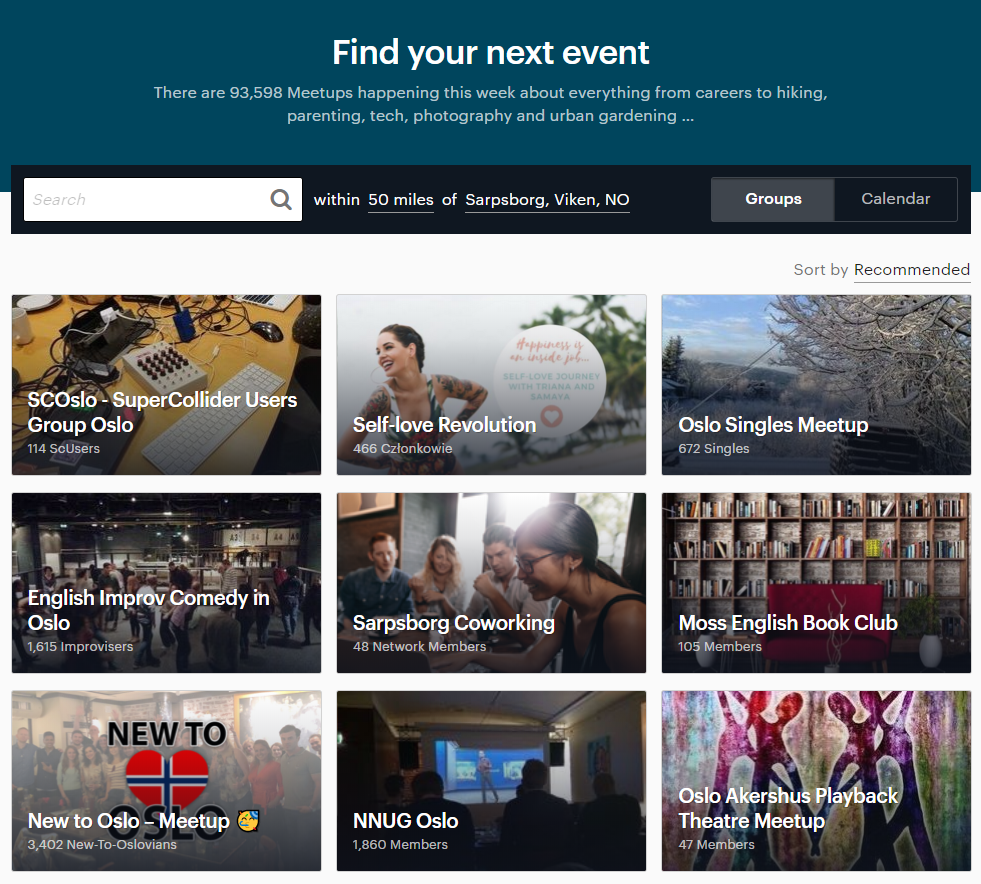
\includegraphics[width=0.48\textwidth]{Illustrasjoner/andre_platformer/meetup_forside.png}
  \end{center}
  \caption{Forsidevisning på Meetup.com etter innlogging.}
\end{wrapfigure}
%END FIGURE%

Etter tvungen brukerregistrering på Meetup.com blir man presentert en forside med en rekke kort som representerer relevante aktiviteter for bruker i geografisk område. 

\vspace{5mm} %5mm vertical space

Ved klikk på et av arrangementene møtes man med en informasjonsside som blant annet informerer om lokasjon, antall medlemmer, organisator, kommende datoer m.m.

\vspace{5mm} %5mm vertical space

I navigasjonen har bruker tilgang på en utforsk-knapp som går til en søkeside, meldinger fra andre brukere og notifikasjoner om relaterte hendelser.

\vspace{5mm} %5mm vertical space

Prosjektgruppen opplever Meetup.com som en nokså ryddig side, dog med minimal aktivitet i Norge. Det er ingen savn etter ytterligere informasjon fra de ulike arrangementene, og det bør bli vurdert lignende implementasjon ved organisasjonssidene som skal utformes på Aktiv Student.

\newpage

NyBy er et verktøy for kommuner og organisasjoner ment for å løse viktige velferdsoppgaver i samarbeid med ansatte og innbyggere\footnote{https://nyby.no/hva-er-nyby}. Kommuner legger ut en henvendelse via meldinger på en app, som medlemmer av frivillige organisasjoner i nærheten kan velge å svare på. Målet er mer direkte kommunikasjon mellom behov og støtte, som igjen vil føre til spart tid og kommunale ressurser.

\vspace{5mm} %5mm vertical space

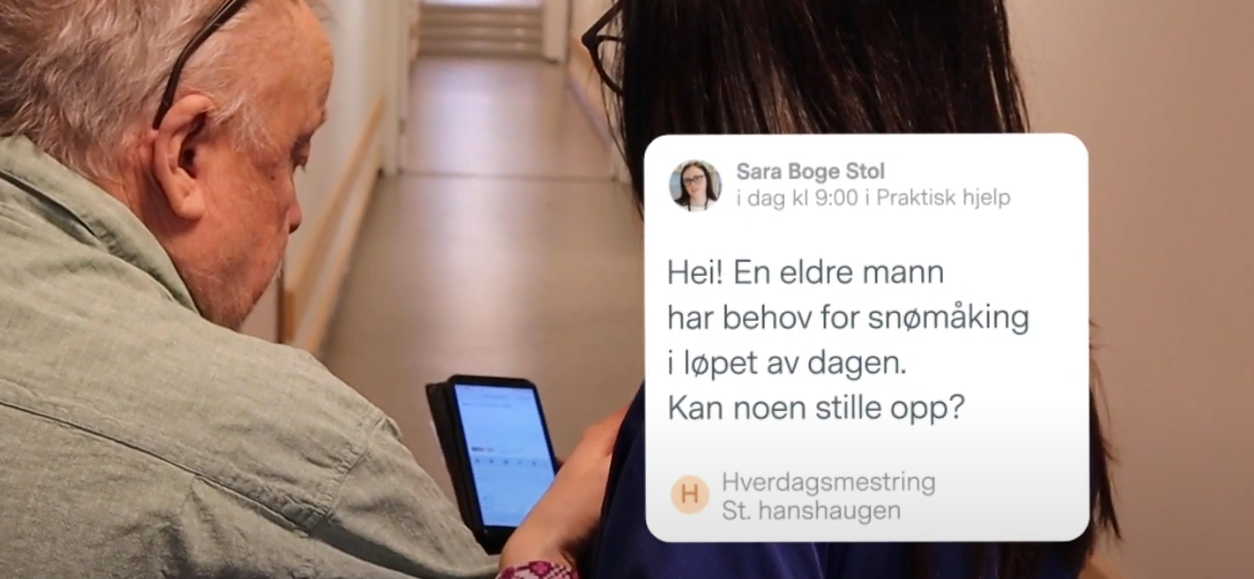
\includegraphics[width=\textwidth]{Illustrasjoner/andre_platformer/nyby_henvendelse.png}

\vspace{5mm} %5mm vertical space
%BEGIN FIGURE%
\begin{wrapfigure}{r}{0.5\textwidth}
  \begin{center}
    
\includegraphics[width=0.48\textwidth]{Illustrasjoner/andre_platformer/nyby_svar.png}
  \end{center}
  \caption{Skjermdump informasjonsvideo fra nyby.no}
\end{wrapfigure}
%END FIGURE%
Via en app kan de som har behov for hjelp melde seg inn i lokale grupper og spørre om bistand til å gjøre mindre ærender. I samme appen kan de som har mulighet til å hjelpe til respondere til den som trenger hjelp.

\vspace{5mm} %5mm vertical space

Prosjektgruppen er imponert over effektiviteten over denne type kommunikasjon ved behov for hjelp. Mange mennesker kan få hjelp til ting som for noen er enkle, men for andre særskilt vanskelig. Dette ved å kutte ut flere ledd innenfor kommunale sektorer, hvor ressursene kan brukes på noe annet. Covid-19 og dens medfølgende karantenetiltak setter desto større fokus på denne type bidrag til samfunnet.

\vspace{5mm} %5mm vertical space

Nextdoor.com setter søkelys på forholdet mellom naboer\footnote{https://global.nextdoor.com/}. Ved registrering kreves verifisering av bostedsadresse, noe som sørger for at brukere kun kan forholde seg til de som bor nær hverandre. Norge er per dags dato ikke et av landene som støttes av Nextdoor, men nettsiden opplyser om et ønske å spre seg til alle land.

\vspace{5mm} %5mm vertical space

Gruppen ser et sterkt fokus på geografisk lokasjon. Selv over nettet så kan miljøet rundt brukere oppfattes veldig personlig, da tjenesten komprimeres kun til de respektive nabolagene.

\vspace{5mm} %5mm vertical space

MeetMe\footnote{https://www.meetme.com/home} og Skout\footnote{https://www.skout.com/} kan sees på som varianter av Tinder, applikasjoner for mennesker i samme geografisk nærområde, som blir definert gjennom fellestrekk i brukerprofilene.

\vspace{5mm} %5mm vertical space

Noe alle evaluerte nettsider har til felles, er at de krever registrering og innlogging. Det foreligger som en naturlig funksjon, da de fleste gjøremål trenger identifisering av bruker. Aktiv Student sitt utgangspunkt er brreg.no, en oversikt over ulike fritidsorganisasjoner, lag og foreninger i Norge. Ved å sammenligne den type innhold med andre oversikter som finnes (finn.no, ut.no, gulesider.no etc), så krever fåtallet av de innlogging. Det forblir da et mål fra prosjektgruppens sin side om å prøve å utelate innlogging, ihvertfall forenkle prosessen betraktelig. Prosjektgruppen diskuterte de forskjellige tjenestene på grunnlag av interessante funksjoner, men også på basis av Jakob Nielsens 10 prinsipper for design av brukergrensesnitt\footnote{https://www.nngroup.com/articles/ten-usability-heuristics/}.

% --------------------- Dette må fullføres ----------------------------- %
\subsection{Relaterte studier og publikasjoner}
De fleste aspektene med oppdraget er forsket på og skrevet om i studier og publikasjoner. Utvikling av søkemotorer og oppslagsverk er gjort før og det finnes nok av dokumentasjon av dette. Prosjektgruppen valgte derfor å trekke fram de mest sentrale aspektene som, når satt sammen, skilte tjenesten beskrevet i oppdraget fra andre tjenester og bidro til at den kunne dekke et behov i markedet. Aspektene som ble trukket fram var {\em gjøre det enklere å delta}, {\em oppfordre til deltakelse sammen med andre}, {\em interaksjon med andre brukere} og {\em foreslå aktiviteter for brukerne}. Disse ble undersøkt nærmere ved hjelp av relaterte studier og publikasjoner.

\paragraph{Gjøre det enklere å delta}
Målet med oppdraget var å lage en tjeneste som gjorde det enklere å finne organisasjoner, lag og foreninger, men for å få noe ut av tjenesten ville det også være helt sentralt å legge opp til at det skulle være enkelt å ta steget for å faktisk delta på aktiviteter. 

Forskningsartikkelen {\em To Go or not to Go!: What Influences Newcomers of Hybrid Communities to Participate Offline} \cite{NEWCOMERS:4:CT17} tar utgangspunkt i tjenesten Meetup, beskrevet i delkapittel~\ref{section:relaterte-tjenester} og~\ref{section:benchmarking}, og undersøkte hvilke faktorer som kunne spille inn for at brukere skulle ta steget til å møte opp på en aktivitet for første gang. Funn fra artikkelen pekte mot flere faktorer som kunne øke sjansen for deltakelse, blant annet {\em utfyllende beskrivelse av arrangementet og instruksjoner for deltakelse
}, {\em at mange andre skulle delta}, {\em inkluderende og velkommende ordbruk i beskrivelsen} og {\em kort sosial distanse mellom bruker og arrangør, slik at det ikke ble truende å ta kontakt}. 

Andre aspekter som kunne vært relevant men som ikke var nevnt i artikkelen var blant annet {\em om vanskeligheter med å finne fram til interessante aktiviteter eller riktig informasjon kunne være en hindring for deltakelse} og om {\em muligheten for å kommunisere med andre potensielle deltakere i et digitalt sosialt felleskap kunne øke sjansen for deltakelse}.

\paragraph{Oppfordre til deltakelse sammen med andre}
Notater:
Det har blitt skrevet om digitale tjenester som oppfordrer brukere til å delta på gruppeaktiviteter i {\em Group-Activity Organizing Through an Awareness-of-Others Interface} \cite{AWARENESS:3:CSCW18}. Artikkelen tar utgangspunkt i en app som lar brukere organisere aktiviteter og andre brukere delta på disse. Fokuset ligger på å gjøre organiseringen og gjennomføringen av aktiviteter så lett som mulig.

\paragraph{Interaksjon med andre brukere}
Notater:
Det er også skrevet artikler om å få ukjente til å ta kontakt med hverandre på digitale tjenester. {\em Outlining the design space of playful interactions between nearby strangers} \cite{NEARBY:5:AM16} beskriver en designprosess med workshops for å utvikle ideer for hvordan fremmede mennesker som befinner seg i nærheten av hverandre kan samhandle på forskjellige måter. {\em Playfulness and progression in technology-enhanced social experiences between nearby strangers} \cite{PLAYFUL:6:NORDICHI18} beskriver videreføringen av denne prosessen, der en app som heter Next2You blir utviklet etter prinsippene fra design-workshops og testet i et bruker-studie. Appen lar brukerne automatisk utveksle valgfri informasjon med andre brukere som kommer innen mobiltelefonens Bluetooth-radius.

\paragraph{Foreslå aktiviteter for brukere}
Notater:
Anbefaling av aktiviteter har blitt skrevet om i artiklene {\em A Novel Method for Event Recommendation in Meetup} \cite{MEETUP:7:ASONAM17} og {\em Users psychological profiles for leisure activity recommendation: user study} \cite{PROFILES:10:CITREC17}. Begge disse artiklene samler inn store mengder informasjon om brukere som brukes til å beregne hvilke aktiviteter som kan være interessante og foreslå disse for brukeren.

\paragraph{Fritid med bistand}
Notater:
Publikasjonene {\em Fritidsorganisasjoner vil og de kan} \cite{FRITID:12}, {\em Inkludering gjennom organiserte fritidsaktiviteter} \cite{INKLUDERING:11} og {\em Tillit, mestring og selvoppfatning} \cite{TILLIT:13} har fokus på aktivisering hos personer med nedsatt funksjonsevne, lav inntekt eller andre tydelige hindringer som gjør at de kan trenge støtte for å delta på aktiviteter. Disse publikasjonene er relatert til Anders Midtsundstad sin metode {\em Fritid med Bistand} \footnote{https://www.fritidmedbistand.no/}. 
% ---------- Annen tittel enn Nye aspekter etc?---------------%
\paragraph{Nye aspekter jobbet med i prosjektoppgaven}
Notater:
Mange av ideéne og prinsippene som er beskrevet i disse artiklene tas med videre av prosjektgruppen i arbeidet med tjenesten. Det er flere aspekter av dette bachelorprosjektet som ikke er beskrevet i publikasjonene nevnt ovenfor. En av disse er autonomi hos brukeren. Et viktig poeng med oppdraget er at brukeren selv skal ville dele informasjon, ta kontakt og delta på aktiviteter. Det vil både være best for brukeren og enklest for utviklingsteamet om brukeren selv velger hvilken informasjon som skal deles. Et annet aspekt som er lite sett på er involveringen av allerede eksisterende organisasjoner og hvordan brukerens deltakelse kan berike både organisasjonene og nærmiljøet sitt. 

I tillegg er det slik at de fleste studiene fokuserer enten på brukere som allerede er sosiale og ikke har problemer med å ta kontakt med andre, eller brukere som har ulike hindringer eller funksjonsnedsettelser som øker terskelen for at de vil ta kontakt eller delta. Ved at målgruppen i dette oppdraget er først og fremst alle studenter ved HIØ vil tjenesten i dette bachelorprosjektet ta hensyn til alle typer mennesker med forskjellige grader av sosiale preferanser, forskjellige motivasjoner, og også personer med forskjellige typer nedsatt funksjonsevne.

\section{Rapportstruktur}
\paragraph{Kapittel 2} inneholder en beskrivelse av arbeidsprosessen med billedlig og skriftlig dokumentasjon, brukerundersøkelser, utvikling av skisser, brukertesting, evalueringer og forbedringer som er gjort.

\paragraph{Kapittel 3}
inneholder en beskrivelse av det det ferdige resultatet som gruppen produserte og en evaluering av dette fra studenter, organisasjoner, fagpersoner og oppdragsgiver.

\paragraph{Kapittel 4}
diskuterer resultatet og om det oppnådde krav og spesifikasjoner satt på forhånd. Her vil det foreligge en vurdering av prosjektet og arbeidet fra prosjektgruppen og anbefalinger og designprinsipper for videre arbeid. Gruppen vil også diskutere erfaringer gjort underveis i arbeidet. Avslutningsvis legges det frem en konklusjon og oppsummering.


    \cleardoublepage
\chapter{Analyse (Generisk tittel)}
\label{chap:analysis}
\meta{
Kapittelet tar for seg analysedelen av arbeidet. Den består av to hoveddeler, en grundig beskrivelse av oppgaven basert på skissen gitt av oppdragsgiver, og en undersøkelse av hva som finnes av relatert arbeid, {\em best practise} og relevant teknologi. 
}

I dette kapittelet danner vi oss et bilde av hvordan en akademisk/teknisk rapport bør se ut, både med hensyn på innhold, struktur og utforming. Vi ser også på hvordan store og komplekse dokumenter blir produsert (både analogt og digitalt), og hva slags (digitale) verktøy som kan tenkes å brukes. Vi går også gjennom endel tilgjengelig materiale som kan gjøre det lettere å velge hva slags digitale verktøy man burde bruke i en bacheloroppgave\footnote{Utvalget er noe overfladisk utført, i hovedsak basert på forfatterens erfaringer.}.  

%\lipsum[3-56]

\section{Beskrivelse av oppgaven}

Løsningen som gruppen har kommet fram til i samråd med oppdragsgiver er et system som bruker informasjon fra Brønnøysundregisteret som grunnlag men i tillegg oppfordrer organisasjoner til å registrere informasjon om seg selv. Målet vil være å utvikle en plattform som er så bra laget og godt markedsført at organisasjonene selv oppsøker den for å registrere informasjonen sin. I oppstartsfasen vil det være nødvendig å ta kontakt med organisasjoner manuelt for å spørre dem om de vil registrere seg. Ved å fokusere på å lage en god algoritme for å finne de mest relevante organisasjonene for sluttbrukeren i Brønnøysundregistreret vil det i tillegg være enkelt å finne ut hvilke bedrifter som er relevant å ta kontakt med for å registrere informasjon i første omgang.


\subsection{Uthenting av informasjon fra Brønnøysundregistret}

\subsection{Registrering av egen informasjon fra organisasjonenes side}

Organisasjoner som registrerer informasjonen sin i plattformen vil bli verifisert og komme høyere opp i søkeresultatene. 

Når de skal registrere informasjon vil de måtte autentisere seg via innlogging, der vil de også huke av for om de godtar kommunikasjon via e-post slik at systemet kan sende påminnelser om å oppdatere informasjon etter X antall måneder.

\subsection{Markedsføring av produktet}

\subsection{Tekniske behov og krav}

Siden systemet inkluderer innlogging og informasjon fra andre kilder enn Brønnøysundregisteret er det behov for en database. 

Systemet har også et administratorpanel der så mye som mulig er automatisert i systemet, slik at det ikke trengs mer enn 5-10 minutter per uke med vedlikehold fra administrator sin side.

\subsection{Produktet som leveres til oppdragsgiver}


\section{Skriveverktøy for store og komplekse dokumenter}

For å starte på et stort og komplekst dokument, vil mange åpne sin vanlige teksteditor og sette igang. Det går sjelden bra. Som ved alle typer større oppgaver, bør man velge sine verktøy med omhu.
Før man setter igang å lage et digitalt dokument, kan det være fornuftig å dvele litt ved hvordan dokumenter har blitt, og blir, produsert på tradisjonelt vis. 

\subsection{Forfatter, redaktør, typograf, trykkeri}

Tradisjonelt hersker det en streng arbeidsdeling innen produksjon av dokumenter, som f.eks. en bok, eller en avis. Forfatteren (eller journalisten) skriver såkalt {\rm brødtekst}, som rett og slett er tekst, skrevet for hånd, på skrivemaskin, eller talt inn på diktafon. I teksten er det gjerne markert ulike strukturelle elementer. Det er markert hvor et nytt avsnitt begynner, kanskje det står skrevet at her kommer det en illustrasjon, etc. Dette råmaterialet går gjerne til en redaktør, som kvalitetssikrer innholdet og tildels struktur, og eventuelt foreslår/foretar endringer. Deretter tar typografen (eller den grafiske formgiveren) over, og bestemmer skriftstørrelser, fonter, marger, linjeavstand etc. Til slutt går trykkoriginalen til trykkeriet\footnote{Her kan jo være på sine plass å tenke litt på XHTML og CSS, og hvor de har sine røtter\dots og da tenker jeg ikke på Håkon Wium Lie \smiley.}.

Denne framgangsmåten ivaretar en klar tredeling av arbeidet; innhold, struktur, og form. Innholdet, og grovstrukturen, bestemmes av forfatteren. Redaktøren sørger for å kvalitetssikre innholdet, og eventuelle justere strukturen. Den endelig formgivingen av dokumentet blir typografens rolle. Det er viktig å merke seg at alle disse tre rollene krever høy kompetanse innen helt forskjellige fagfelt. De fleste mener også at det er ganske unaturlig for en forfatter å legge ned mye tankearbeid i hvilken font og størrelse det bør være på overskriftene. På den annen side ville vel det ikke være rett at typografen blandet seg bort i innholdet.

\subsection{The curse of the cursor \\  \normalsize -eller- \\DTP: DeskTop Publishing eller Dom Tokigas Paradis? }

Og etterhvert kom datamaskinene, som tilsynelatende kunne gjøre ``alt'', og dermed begynte mange å gjøre ``alt'', selv. Teksteditorer og desktop publishing verktøy gjorde det mulig for at en person kunne stå for hele prosessen, både skrive, redigere, og formgi, uten å ha særlig kompetanse, ferdighet eller erfaring i noen av feltene.

Personlig husker jeg godt mitt første møte med DTP, tidlig i IT-utdannelsen. Oppgaven var å lage en liten avis, med bilder og det hele, ved hjelp av en søt liten Mac, som på et mysteriøst vis var knyttet sammen med en skriver som til og med skrev ut illustrasjoner og fotografier i grov oppløsning. Den blinkende markøren i teksteditoren var hypnotisk, halvt innbydende, halvt skremmende. Og så måtte man bare kaste seg ut i det. Skrive noen setninger, markere en del som ``bold'' og fontstørrelse 18, fin overskrift, et par ``enter'', forsette med vanlig font, nei, kanskje en litt mer fancy kalligrafifont, kanskje til og med blå? Og dermed var det gjort, forvirringen var total. Noe senere erfarte jeg at i enkelte svenske miljøer mente man at DTP sto for ``Dom Tokigas Paradis". Innen visse segmenter av reklamebransjen mener jeg fremdeles å se spor etter slike traumatiske møter med datastøttet publisering.

Man kan jo spørre seg om det egentlig er noen forskjell mellom et blankt ark, enten på et skrivebord eller i en skrivemaskin, og en blinkende markør øverst i venstre hjørne i en editor? Uansett svar, det blanke arket gir deg ikke anledning til å eksperimentere med fonter, marger, skriftstørrelse og plassering av bilder. Arket handler kun om innhold, og hvordan det skal struktureres, hvilken passasje som følger en annen, og hvor det begynner et nytt avsnitt.

\subsection{Programmering av dokumenter}

Et par år senere skal jeg produsere min første akademiske artikkel, i \LaTeX~med  AMS stilen. Hæh?

Det tok et par dager før jeg skjønte poenget. Skrive innholdet i filer (ark) i en editor uten formateringsmulighet, sette inn kryptiske kommandoer for å markere avsnitt eller matematiske uttrykk, sette sammen delene i en styrefil, legge til noen kommandoer som avgjorde hvordan dokumentet ble seendes ut. Deretter {\em kompilere} hele greia! Som så resulterte i  en DVI-fil\footnote{DVI: DeVice Independent}, som igjen kunne konverteres til alle mulige trykk- og printbare formater. Og det beste av alt, resultatet, rent formmessig, ble helt strøkent, akkurat som i lærebøkene og artikkelsamlingene.

Dette var jo akkurat som å programmere. Full kontroll.


\section{Digital dokumentproduksjon}

Vi foreslår et sett med minimumskrav til digitale dokumentverktøy, basert på  den forutgående analysen. Deretter gir vi kort beskrivelse av 
\LaTeX~ og OpenOffice Writer, som etter en kort vurdering er de to verktøyene som tilfredstiller de fleste av kravene.

\subsection{Generelle krav}
\label{sec:generelle-krav}

Kravene er utarbeidet delvis med basis i den forutgående analysen, men i hovedsak ut fra forfatterens erfaringer.

\vspace{1em}
\begin{compactdesc}
\item [Plattformuavhengighet] I et prosjekt med flere deltagere, er det direkte arrogant å forvente at alle skal bruke samme plattform, fordi valget av dokumentasjonsverktøy krever dette.
\item [Robusthet] En hovedrapport er ofte relativt stor, og tildels med komplekst innhold (figurer, tabeller etc). Det er ikke uvanlig at selv kostbare og vidt utbredte verktøy kræsjer i en slik kontekst, eller verre, begynner å oppføre seg inkonsistent og uforutsigbart Det å åpne et dokument, bare for å oppleve at formatering som ble foretatt kvelden før er ødelagt, er ingen særlig givende erfaring, særlig ikke hvis det er to timer til rapporten skal leveres inn.
\item [Maler/stiler] Det må kunne være mulig å skifte mal på et og samme dokument uten å gjøre ekstra tilpasninger. Dermed oppnår man et klart skille mellom innhold og utforming. Hvis f.eks. retningslinjene for hovedrapporten endrer seg, så er det bare å lage en ny mal og bruke denne.
\item [Oppsplitting]Det bør kunne være mulig å splitte dokumentet i mindre deler, f.eks. en fil for hvert kapittel. Delene må kunne knyttes sammen i et masterdokument. På denne måten vil det være lett å endre rekkefølgen på komponentene. Da er også strukturen uavhengig av det faktiske innholdet. Oppsplitting er også en forutsetning for å kunne jobbe distribuert, der de ulike deltagerne jobber parallelt på ulike deler av rapporten.
\item [Kryssreferanser]Det må være mulig å bruke dynamiske kryssreferanser, slik at man f.eks. kan referere til en nummerert figur. Hvis da nummeret til figuren endrer seg pga. av at det blir lagt inn en figur tidligere i dokumentet, så må referanse oppdateres automatisk.
\item [Bibliografi]De må være enkelt å referere til en ekstern samling bibliografiske referanser. Det også være enkelt å når som helst endre referansestil (f.eks. IEEE eller Harvard).
\item [Brukermasse]Det bør eksistere en stor og variert brukermasse, noe som i seg selv kan være en antydning om at verktøyet holder mål.
\item [Dokumentasjon]Verktøyet må være godt dokumentert, både den innebyggede dokumentasjonen, samt i ulike fora på nettet.
\item [Versjonskontroll]Det må være enkelt å håndtere versjonering, dvs. at man lett kan rekonstruere tidlige versjoner, og lett se hva som er endret fra versjon til versjon.
\item [Framtids/fortidssikker]Verktøyet bør kunne uten videre behandle dokumenter som er laget i tidligere versjoner. Dette vil også være en indikasjon på at dokumentet du jobber fremdeles ``lever'' i rimelig overskuelig framtid. 
\item [Stave/grammatikkontroll] Minimumskravet er at det er mulig å utføre effektiv stavekontroll, for ulike språk, ikke minst norsk bokmål. I tillegg vil det være et pluss om det er mulig å verifisere grammatikk.
\end{compactdesc}


\subsection{\LaTeX}

Klipt og limt fra Wikipedia\footnote{\url{http://no.wikipedia.org/wiki/LaTeX}}:

\begin{quotation}
\LaTeX~ er et typesettingssystem for dokumentproduksjon. Det skrives normalt LaTeX i dokumenter som ikke har hevet og senket tekst.
\LaTeX~ ble opprinnelig utviklet av Leslie Lamport i 1984 og tilbyr idag en lang rekke dokumentproduksjonspakker som f.eks. automatisk opprettelse av innholdsfortegnelser, lister med tabeller og figurer, inkludering av bilder, kryssreferanser, sideoppsett, bibliografier mm.


LaTeX~ baserer seg på at forfatteren av et dokument kun skal være forfatter av dokumentet og slippe å bry seg om utforming og hvordan ting ser ut; noe han normalt sett ikke er ekspert på uansett. Det forfatteren gjør er å dele opp dokumentet i logiske strukturer før han lar LaTeX~ ta seg av selve oppsettet. LaTeX~ ansees ofte som WYSIWYM (det du ser er det du mener) fremfor WYSIWYG (det du ser er det du får) editor. Dette fører til at det ofte anerkjennes som overlegent fremfor andre skriveprogrammer grunnet at endringer som påvirker hele dokumentet er meget enkle å gjennomføre. De trenger ofte bare en endring et sted, så er endringen gjennomført i hele dokumentet.
\end{quotation}


\subsection{OpenOffice Writer (med kloner)}

Klipt og limt fra Wikipedia\footnote{\url{http://no.wikipedia.org/wiki/OpenOffice}}:

\begin{quotation}
Apache OpenOffice (AOO), er en kontorprogramvare som inneholder tekstbehandlingsprogram, regneark, presentasjonsprogram, tegneprogram og et databaseprogram. AOO er fri programvare, og distribueres av Apache Software Foundation under Apache-lisensen. Det betyr at både programmet og dets kildekode kan lastes ned gratis, og privatpersoner eller bedrifter kan selv gjøre endringer eller reparere feil. 

AOO benytter ODF som sitt primære dokumentformat. Dette er en ISO-standard som blant annet er tatt i bruk av offentlig sektor i Norge og EU for utveksling av digitale dokumenter. I tillegg støttes formatene til Microsoft Office og en rekke andre kontorprogrammer. AOO er multiplattform programvare, tilgjengelig for mange forskjellige operativsystemer, deriblant Microsoft Windows, Mac OS X, Linux, Solaris, FreeBSD, NetBSD og OpenBSD.
\end{quotation}


    \cleardoublepage
\chapter{Design / Utforming/ Planlegging (Generisk tittel)}
\label{chap:design} 
\meta{
 Basert på beskrivelsen av oppgaven (Avsnitt \ref{sec:oppgaven}) og analysen i (Kapittel \ref{chap:analysis}), skal denne delen beskrive hvordan man har tenkt å utforme løsningen. Beskrivelsen er noe avhengig av type prosjekt.
 

\paragraph{Utredning}

Først og fremst må det redegjøres for hvordan man skal innhente informasjonen som skal danne grunnlaget for utredningen. Deretter må man bestemme hvordan man skal behandle materialet, f.eks. om man skal bruke statistiske metoder. Etter det er det naturlig å presentere en disposisjon for selve utredningen, som i dette tilfellet vil være hovedresultatet i prosjektet. Selve utredningen bør være et frittstående dokument, på samme måte som en film vil være et frittstående dokument i en mediaproduksjon, og et program vil være i et utviklingsprosjekt.

\paragraph{Mediaproduksjon}
Her vil det være naturlig å presentere story-boards og liknende metoder for å beskrive produksjonen. 

\paragraph{Utvikling}
Her er det bare å ta for seg av ulike måter å beskrive systemer på, alt fra overordnet arkitektur, moduler, meldingsprotokoller etc. Bruk gjerne formelle beskrivelsesspråk, typisk UML. 
}

I det videre tar vi for oss oppgaven med å utvikle struktur, innhold og formgiving av rapportmalen, uavhengig av hvilket verktøy som skal brukes ved implementasjonen.


\section{Struktur}

Vi tar utgangspunkt i den tradisjonelle og generiske strukturen beskrevet i Avsnitt \ref{sec:mayfield}. Det er etter min mening vanskelig å se noen grunn til å gjøre noe annet.

\section{Innhold}

Vi så Avsnitt \ref{sec:hiof-it}  at man ved HiØ skiller mellom produkt- og prosessdokumentasjon, og operer med flere frittstående dokumenter. Det er ønskelig at hovedokumentet omhandler løsningen av oppdraget, dvs. selve produktet.
Struktur og innhold bør være som som følger:

\begin{compactdesc}
\item [Front Matter]  Som i Avsnitt \ref{sec:mayfield}.

\item [Body] Hoveddelen av dokumentet (gjennomføringen).
\begin{compactdesc}
\item [Introduksjon] Skal gi leseren et bilde av rammene rundt prosjektet: Kort beskrivelse av oppdraget, litt om oppdragsgiver og prosjektgruppen, prosjektets formål, leveranser og metoder. Den bør også inneholde en oversikt over resten av rapporten. 
\item [Analyse] Kapittelet tar for seg analysedelen av arbeidet. Den består av to hoveddeler, en grundig beskrivelse av oppgaven basert på skissen gitt av oppdragsgiver, og en undersøkelse av hva som finnes av relatert arbeid, {\em best practise} og relevant teknologi. 
\item [Design]  Basert på beskrivelsen av oppgaven i introduksjonen  og analysen, skal denne delen beskrive hvordan man har tenkt å utforme løsningen. Beskrivelsen er nødvendigvis noe avhengig av type prosjekt. Designet er uavhengig hva slags verktøy man skal bruke i implementasjonen.
\item [Implementasjon] Her skal det beskrives hvordan man faktisk produserte leveransene i prosjektet, og viktigst, beskrive selve produktet. Hvilke verktøy brukte man, hvordan foregikk produksjonen, etc. Utformingen av dette kapittelet avhenger helt klart av type prosjekt.
\item [Evaluering] De fleste prosjekter avsluttes med en eller annen form for evaluering av resultatene. I utviklingsprosjekter vil det være naturlig med teknisk testing, fungerer programvaren som den skal? Teknisk testing kan utføres av utviklerne selv, eller en ekstern part, f.eks. oppdragsgiver. En oppdragsgiver ønsker ofte å utføre en akseptansetest, dvs. en test som vil avgjøre om de har "fått det de har betalt for". Ellers vil det i mange tilfeller være nyttig og viktig med en brukertest, dvs. en strukturert test der sluttbrukerne får komme til orde. 
\item [Diskusjon] Diskusjonskapittelet er viktig, både for dere selv og sensor. Dette kapitelet er det som i hovedsak skiller et akademisk prosjekt fra et rent næringslivsprosjekt. Ble resultatet som forventet? Ble oppdragsgiver fornøyd? Kunne dere gjort noe anderledes/bedre?
Det er her dere skal dokumentere at dere har lært noe underveis, ikke bare levert et produkt til en oppdragsgiver. 
\item [Konklusjon] Konklusjon er på et vis et sammendrag av diskusjonskapittelet. Her bør dere legge vekt på de viktigste funnene, både når det gjelder produktet og prosessen. Med et fyldig diskusjonskapittel bør trenger ikke konklusjonen bør være mer enn en side.
\end{compactdesc}

\item [Back Matter] Som i Avsnitt \ref{sec:mayfield}.

\end{compactdesc}

\section{Utformingen}

Det følger med en del standard, ferdig definerte stiler med enhver \LaTeX~distribusjon. Disse er gjennomprøvet over flere 10-år, og har tålt tidens tann både teknisk og estetisk. Når man skal lage sine egne design, vil det som regel alltid være fornuftig å gå ut i fra en  av standardstilene. Det gjør vi også i dette prosjektet, og tar utgangspunkt i stilen {\em report}, parametrisert for dobbeltsidig A4-format, med 11pt basis fontstørrelse. Vi foreslår følgende endringer i report-stilen: 

\paragraph{Marger}
I følge egen og kollegers erfaring er marginene noe store i standardrapporten, slik at det blir litt ``trangt'' for tekst, tabeller og illustrasjoner. Vi foreslår en layout med reduserte marger på alle sider.


\paragraph{Topptekst / bunntekst}
Når man slår opp en dobbeltsidig bok, kalles venstre side for {\em verso}, og høyre for {\em recto}.
\index{Recto}
Vi ønsker at bunnteksten skal være uten andre elementer enn fotnoter. Sidetallet bør trykkes i toppteksten, til venstre på verso sider, og til høyre på recto sider. På denne måten
blir det lett å bla fort igjen for å finne et gitt sidetall,  som f.eks. er funnet i en indeks. Videre er det ønskelig at aktuelt kapittel er angitt til høyre på verso sidene, og aktuelt underkapittel til venstre på recto sidene.

\paragraph{Tittelsiden} 
Det skal være to tittelsider, først en fengende forside, som studentene utformer selv, og deretter en standard bacheloroppgave-side som er lik for alle.


\section{Leveransene og malen}
Første versjon av hoveddokumentet  bør bestå av introduksjonen og analyse- og designkapitlene (Kapittel \ref{chap:intro}, \ref{chap:analysis} og Kapittel \ref{chap:design}), og andre versjon bør være en mer eller mindre komplett beskrivelse av selve resultatet (Kapittel \ref{chap:implementation}). Endelig leveranse tilsvarer den komplette rapporten pluss selve produktet (og poster og presentasjon).






    \cleardoublepage
\chapter{Implementasjon / Produksjon / Gjennomføring (Generisk tittel)}
\label{chap:implementation} 

\meta{
Her skal det beskrives hvordan man faktisk produserte resultatene i prosjektet, og viktigst, beskrive selve produktet. Hvilke verktøy brukte man, hvordan foregikk produksjonen, etc. Utformingen av dette kapittelet avhenger helt klart av type prosjekt.
}

\section{Utredning}

\meta{
Det er mulig at dette kapitellet er overflødig i et utredningsprosjekt. Utredningen er jo et eget dokument, og trenger vel ikke med kontekst for å kunne evalueres.
}

\section{Mediaproduksjon}

\meta{
For denne typen prosjekter kan det være relevant å beskrive og rapportere fra selve produksjonen. Det er vel relativt vanlig at man må endre og improvisere i forhold til opprinnelig plan, og det bør jo absolutt dokumenteres, ikke minst i forhold til diskusjonen (Kapittel 6.2). er mulig at dette kapitellet er overflødig i et utredningsprosjekt. Utredningen er jo et eget dokument, og trenger vel ikke med kontekst for å kunne evalueres.
}

\section{OpenOffice Writer}

Se vedlegg i rapporten {\em OpenOffice mal for hovedprosjektrapport}.

\section{\LaTeX}

For et nærmere innblikk i hvordan denne malen er implementert, se kildekoden som følger med.
Resultatet av den ønskede layout kan selvfølgelig sees i dokumentet du leser nå, eller i mer formell form i Figur \ref{fig:layout1}.


\begin{figure} 
\index{Recto} 
\printinunitsof{mm}
\currentpage
\oddpagelayouttrue
%\oddpagelayoutfalse 
%\twocolumnlayouttrue 
\pagediagram 
%\drawpage
%\pagedesign
\center
\setvaluestextsize{\scriptsize}
\pagevalues
\caption{Layout for recto sider} 
\label{fig:layout1} 
\end{figure}

    \cleardoublepage
\chapter{Testing / Evaluering (Generisk Tittel)}
\label{chap:evaluation} 
\meta{
De fleste prosjekter avsluttes med en eller annen form for evaluering av resultatene fra prosjektene. I utviklingsprosjekter vil det være naturlig med teknisk testing, fungerer programvaren som den skal? Teknisk testing kan utføres av utviklerne selv, eller en ekstern part, f.eks. oppdragsgiver. En oppdragsgiver ønsker ofte å utføre en akseptansetest, dvs. en test som vil avgjøre om de har "fått det de har betalt for". Ellers vil det i mange tilfeller være nyttig og viktig med en brukertest, dvs. en strukturert test der sluttbrukerne får komme til orde.

Evalueringsmetoden vil altså avhenge sterkt av typen av prosjekt. Likevel vil de samme overordnete prinsippene gjelde for alle typer leveranser. En utredning bør kunne passere en akseptansetest, et mediaprosjekt bør kunne underlegges både akseptanse- og brukertest (jfr. kritikerprosessen rundt nye spillefilmer), og et programvareprosjekt bør i tillegg gjennomgå en teknisk test.
}



Testingen av de to verktøyene er utført på en uformell og ikke særlig vitenskapelig basert måte, og resultatene baserer seg hovedsakelig på forfatterens egne vurderinger\footnote{I et reelt prosjekt ville denne metoden være litt for tynn \smiley}.

I Tabell \ref{tab:comparison} er det foretatt en summarisk sammenlikning mellom OpenOffice og \LaTeX~ med hensyn på kravene i Kapittel \ref{sec:generelle-krav}.


\begin {table}[h!]

\begin{center}
\begin{longtable}{|l|p{0.332\textwidth}|p{0.33\textwidth}|}
\hline
 {\bf Krav} & {\bf OpenOffice} & {\bf \LaTeX} \\ 
\hline
Robusthet & Tildels betapreget. Man har av og til følelsen av å bevege seg på  tynn is. & Bunnsolid, Gigabyte type dokumenter ingen problemer.\\ 
\hline
Åpne formater &
Ja. En ODF fil er en zipfil som inneholder en rekke skjemadefinerte XML filer. &
Ren, ``lettlest'' ASCII.\\ 
\hline
Maler/stiler &
Ja, men noe rotete, lett å overstyre lokalt uten at du merker det. &
LaTex ``oppfant'' prinsippet med å skille innhold, struktur og presentasjon. Enormt tilfang av maler og stiler for det meste.\\ 
\hline
Oppsplitting &
Mulig, men ikke trivielt/robust. &
Trivielt. Modus Operandi for store dokumenter, f.eks. Proceedings som samler ``stand-alone''-artikler fra mange forfattere.\\ 
\hline
Kryssreferanser &
Går greit, men ikke helt intuitivt. &
Konsistent og enkelt.\\ 
\hline
Bibliografi &
Greit med bruk plugins/extensions, f. eks, Zotero. &
BibTex innførte prinsippet om å referere til eksterne bibliografisamlinger. En mengde ulike stiler.\\ 
\hline
Brukermasse &
Stadig økende, men med stort innslag av entusiaster og ``pionerer''. &
Stor og kompetent, særlig innen den naturvitenskapelige og tekniske delen av akademia.\\ 
\hline
Dokumentasjon &
Relativt god, men bærer preg av at produktet er ``ferskt''. &
Meget omfattende, men godt spredt i ulike fora.\\ 
\hline
Versjonering &
En odf-fil er en binærfil (zippet og komprimert samling XML-dokumenter), og egner seg dårlig for tradisjonell versjonskontroll. Det finnes en innebygget versjonerings-mekanisme, men det er usikkert hvor hensiktsmessig denne er.&
Filene er ren ASCII, og håndteres derfor trivielt i alle typer versjoneringssystemer.\\ 
\hline
Framtidssikker &
Uklart, siden det er et ``ferskt'' verktøy, men potensialet er der.&
Kan ikke bli bedre? Egen erfaring med komplekse og store dokumenter fra tidlig 90-tall som problemløst kan  behandles i dagens verktøy.\\ 
\hline
Staving/grammatikk &
Innebygget, mulig å laste inn ulike typer eksterne ordlister etc.&
Mange vektøy, fordi filene er ren ASCII.\\ 
\hline
\end {longtable}
\caption {Summarisk vurdering av sentrale aspekter i OpenOffice og \LaTeX~\label{tab:comparison} }
\end{center}
\end {table}






    \cleardoublepage
\chapter{Diskusjon}
\label{chap:discussion} 

I dette kapittelet vil resultatet bli diskutert. Kapittelet vil fokusere på om resultatet ble som forventet, om oppdragsgiver var fornøyd med resultatet, om gruppen gjort noe annerledes/bedre og hva gruppen har lært underveis. Det vil også inneholde en vurdering av produktet opp mot relatert arbeid. Gruppen vil gi anbefalinger og fremlegge designprinsipper for videre arbeid og utvikling av plattformen i praksis. Til slutt er en konklusjon med oppsummering av arbeidet og prosessen.

\section{Resultat i forhold til prosjektbeskrivelse}
\hl{Nye notater}
Notater:
Ble ikke utviklet en funksjon for å hente inn informasjon om organisasjoner.
La til sosialt aspekt/kommunikasjon mellom brukere.
La til kartleggingstest/forslag til aktiviteter for brukere.
Har laget noe mer enn det prosjektbeskrivelsen foreslo.

\section{Resultat i forhold til sluttbrukerens krav}

\section{Gruppens evaluering}

\section{Erfaringer gjort underveis}
\hl{Nye notater}
Notater:
Digitalt gruppearbeid.
Gjennomføring av brukerundersøkelser i et større prosjekt.
Oppsett og struktur på større faglige oppgaver.
Tverrfaglig prosjektarbeid.
Verdien av å konsultere fagpersoner og eksperter, samt hvordan finne disse.
Hvordan forholde oss til og samarbeide med en oppdragsgiver.
Finne løsninger som fungerer som en middelvei mellom forskjellige ønsker.
Systematisk problemløsing.
Selvstendig planlegging og utførelse av en brukerorientert designprosess.
Akademisk skriving.
Selvstendig utforming av krav til produkt.

\subsection{Hva kunne blitt gjort annerledes?}
\hl{Nye notater}
Notater: presentere 3 ulike løsninger til oppdragsgiver, utforsket aspektet om drift av selve tjenesten, tekniske løsninger for drift, prøvd å ha flere deltakere for brukerundersøkelser, tatt kontakt med komunner og frivillighetssentralen tidligere, tatt kontakt med Anders Midtsundstad tidligere for slutt evaluering av konseptet.

\section{Anbefalinger for utvikling og videre arbeid}
\label{section:anbefaling-videre-utvikling}

\subsection{Tekniske avhengigheter}
\hl{Endringer}

\paragraph{Feide og tilgang til studentinformasjon}
\hl{Nytt avsnitt}
Notater:
Hvorfor bør tjenesten ha Feide?
Samtale med Feide, virket ikke som en hindring.
Fikk ikke svar fra IT-drift.
Utfordring med sikkerhet, høgskolen er selv ansvarlig.
Drøfting og vurdering av alternativer til Feide.

\paragraph{Database}
Siden systemet inkluderer innlogging og informasjon om organisasjoner fra andre kilder enn Brønnøysundregisteret vil det være behov for en database som kan lagre informasjon om både brukere, organisasjoner og administrator. \hl{Om Feide-innlogging implementeres og dette i tillegg kan brukes til å hente ut informasjon om studenten som logger inn fra HIØ sine datakilder, trengs ikke informasjon om studenter som passord, e-post og navn å lagres i systemets database. Om studenten velger å legge til ytterligere informasjon til profilen sin, som organisasjoner og aktiviteter den er interessert i, beskrivelse eller bosted, vil det være hensiktsmessig å kunne lagre dette i systemets database sammen med en ID knyttet opp mot studenten.}

\paragraph{Publiseringsløsning}
\hl{Nytt avsnitt}
Notater:
Vurdere og drøfte ulike publiseringsløsninger: Wordpress eller lignende CMS, plugin eller nettsted, Vortex (HIØ sitt CMS), app, kode eget rammeverk.

\subsection{Utvikling av tjenesten}
\hl{Nytt avsnitt}
Notater:
Vurdering og drøfting av alternativer: bachelorprosjekt, masterprosjekt, outsourcing, delvis outsourcing, samarbeid med kommunen(e).
Kan søke om midler til utvikling.

\subsection{Drift av tjenesten}
\hl{Nytt avsnitt}
Notater: 
Tar veldig mye tid å gjøre manuelt, 100 telefoner/mailer i måneden + fikse løpende hendelser
Presenter flere aktuelle løsninger: webcrawler, egen stilling, halvautomatisering, outsourcing

\subsection{Merkevarebygging og synliggjøring av produktet}
\hl{Endringer}
Prototypen til tjenesten Aktiv Student ble utformet på oppdrag fra HIØ som et av deres bachelorprosjekter. Dette alene kan styrke tjenestens troverdighet blant potensielle brukere og eventuelt andre interesserte aktører, enda mer om HIØ offentlig stiller seg bak tjenesten ved å for eksempel integrere det som en del av sin hjemmeside.

\paragraph{Utfordringer}
Utfordringen blir å skape et levende produkt, hvor organisasjoner legger inn egen informasjon og sørger for at ny og oppdatert informasjon blir lagt til kontinuerlig. Dette innebærer at det må være attraktivt for organisasjoner og legge til informasjon og oppdatere sine sider inne på plattformen.

\hl{Notater:
Stor utfordring blir å få i gang plattformen med de første få brukerne.} \say{\hl{Users can be motivated in multiple ways—through rewards, through a clear understanding of what an application offers them, and through delivering what they want in the fastest, best way possible.}} (s.123) \cite{INTERACTIVE-DESIGN:19}.

\hl{Få brukere motivert til å logge inn/opprette brukerkonto og ikke bare passivt bruke tjenesten.

Passe på at tjenesten ikke dør ut, kontinuerlig markedsføring, hvert nye studiekull, nye organisasjoner, oppdatert informasjon, drift, aktivitet i sosiale medier og på høgskolens nettside, skriv ned noen markedsføringsprinsipper for å sikre at brukere kommer tilbake og fortsetter å bruke tjenesten, og at nye brukere også kommer. Utfordring om studenter slutter på skolen men fortsatt står i listen over interesserte studenter, kan ødelegge troverdigheten til denne funksjonen om folk ser at mange av de som står der ikke egentlig er med}

\paragraph{Hvordan kan dette løses?}

Produktet må være godt synlig og lett tilgjengelig plassert på fremsiden til Høgskolen i Østfold for at dette produktet skal bli brukt av studenter. det anbefalles også at det blir kjørt et redesign av HIØ sitt nettsted ettersom det er ganske kaotisk på nåværende tidspunkt. For at det skal være attraktivt for organisasjoner å legge inn og oppdatere sin informasjon så skal det introduseres ett system som plasserer organisasjoner med oppdatert informasjon lengre opp på resultat listene. I tillegg skal det i start fasen av produktet kontaktes en del store organisasjoner for å få de til å legge til informasjon om seg selv som igjen kan starte et initiativ hos andre til å legge til sin informasjon. 


\paragraph{Synliggjøring opp mot studenter}

\hl{Nytt avsnitt}
Dette produktet er laget for nye studenter ved høgskolen og skal hjelpe dem i starten av studie tiden for å finne fritids aktiviteter og organisasjoner å ta del i. Resultater i våre brukertester og undersøkelser viser at dette er noe nåværende studenter ønsker fantes da de startet, og noe kommende studenter sier hadde vært et bra tiltak for dem når de skal studere. 
undersøkelsene våre viser at dette produktet er noe som må introduseres så tidlig som mulig i studietiden. gruppens hovedtips til utviklere og administrator er at dette produktet må ha en sentral rolle på høgskolens nettside, introduseres i fadderukene og markedsføres gjennom student politikken og student organisasjoner.

\paragraph{Markedsføring opp mot organisasjoner}

\hl{Nytt avsnitt}
Markedsføringen opp mot organisasjoner i starten er en god del manuell jobb for administrator for dette produktet hvor administrator selv må sende ut invitasjoner og rekrutere organisasjoner til siden. Derfor er det viktig for utviklere og automatisere så mye av prosessen når det kommer til rekruttering som mulig. Men all jobben som legges ned i oppstarten av dette produktet vil være vel verdt det etterhvert når produktet blir mer kjent blant organisasjoner å de selv kommer til siden for å registrere seg. Etterhvert når merkevaren blir godt kjent og kanskje har spred seg ved å bli tilbudt eller tatt opp av andre instanser, håper vi at dette vil skape en type bevegelse blant organisasjoner i Norge hvor det å være en del av merkevaren "Aktiv Student" er attraktivt og hjelper til å berike organisasjons samfunnene og nærområdene rundt. Gruppens hovedtips for utviklere og administrator er å starte med studentorganisasjonene å få med alle disse så det vises at høgskolen stiller seg bak. Noe som kan hjelpe merkevarebyggningen kraftig er å presentere dette produktet for de forskjellige organisasjons forbundene i Norge å få dem ombord, så de kan markedsføre dette videre til sine organisasjoner. Prøv å skape media dekking rundt merkevaren for å introdusere dette til nærmiljøet. 

\subsection{Mulighet for utvidelse av tjenesten}
\hl{endringer}
Som en del av oppdraget ble tjenesten utviklet i hovedsak for HIØ. Men etter oppdragsgivers ønske er også muligheter for utvidelse av tjenesten til bruk for andre aktører utforsket. Informasjonen om lag, foreninger og organisasjoner som ligger tilgjengelig på Brønnøysundregisterets API dekker hele Norge. Det betyr at systemet kan enkelt få tilgang på all denne informasjonen. Ved noen enkle endringer i parameterene i systemets kode kan tjenesten tilbys til for eksempel andre høyskoler, kommuner, fylkeskommuner og andre interesserte aktører. \hl{Ved bruk av aktører utenfor sektor for høyere utdanning vil Feide-innlogging måtte erstattes eller suppleres med andre løsninger, det vil være aktuelt å undersøke løsninger som for eksempel MinID \footnote{http://eid.difi.no/nb/minid} eller BankID \footnote{https://www.bankid.no/bedrift/}.} Ved å tilby tjenesten til større aktører kan dette også bidra til å skape et større navn for tjenesten, som igjen kan bidra til å synliggjøre tjenesten og skape mer tillit overfor organisasjoner og privatbrukere, øke antall brukere og skape en god sirkel av merkevarebygging for alle parter.

\paragraph{Løsninger for kommersialisering}
\hl{Nytt avsnitt}
Notater:
Kommunen, kickstarter, søke bidrag for folkehelsefremmende/samfunnsbyggende arbeid, private investorer, andre utdanningsinstitusjoner. Hvordan får man hjulet til å rulle, få nok brukere slik at man vet at det fungerer før man selger det videre. Lisens på 50k i året, ha en 50-100\% stilling på drift.
%den her er jeg litt usikker på hvordan jeg skal skrive%

\paragraph{Markedsføring opp mot potensielle kunder eller investorer}
\hl{Nytt avsnitt}
Notater:
Folkehelse, mer effektiv i arbeid, samfunnsbygging, tilhørighet til kommunene, studenter melder flytting, bryr seg mer om stedet de bor og bidrar i samfunnet, frivillighet får alt til å gå rundt, kompetansetilflyttere får tilknytning og blir.

Studier viser oss at det å være i fysisk aktivitet eller det å ha en hobby bidrar til blant annet: bedret folkehelse, mer effektivitet i arbeidslivet, økt selvfølelse av tilhørlighet,bedre samfunns velferdsel og bedre personlig selvfølelse. For å få denne tjenesten ut i liv, som noe som kan bidra til disse punktene blant samfunn som kommuner, skoler og andre nærmiljø er det viktig at det blir markedsført på en måte som drar frem disse mulige verdiene. Når dette blir pitchet til potensielle kunder og investorer er det viktig å vise at denne tjeneste ikke bare tilbyr et produkt som operetter bedre kommunikasjon mellom samfunn og organisasjoner, men at det muligens kan dra frem disse verdiene å føre til et bedre samfunn i sin helhet.


\section{Konklusjon og oppsummering}
Coming soon to a hoveddokument near you







    \cleardoublepage
\chapter{Konklusjon}
\label{chap:conclusion} 
\meta{
Konklusjon er på et vis et sammendrag av diskusjonskapittelet. Her bør dere legge vekt på de viktigste funnene. Med et fyldig diskusjonskapittel bør trenger ikke konklusjonen bør være mer enn en side, men legg vekt på tydelig og godt språk. Husk at sensor antagelig først leser sammedraget, deretter konklusjonen. Etter det står resten av dokumentet for tur.
Fokuser på hvordan produktet ble i forhold til forventningene til oppdragsgiver og dere selv. Gjenta i kortform de viktigste punktene fra diskusjonskapitlet. I tillegg bør dere nå se videre, om hva som burde bli gjort ved en videreføring av prosjektet (framtidig arbeid). I tillegg kan dere her gi råd om videre arbeid.
}

Prosjektet har demonstrert at det er mulig å lage maler for hovedrapporten i bachelorprosjektet ved HiØ/IT i både OpenOffice og\LaTeX. Malene tilfredstiller kravene til struktur og utforming, og tilbyr nødvendig funksjonalitet. Det er imidlertid åpenbart at at \LaTeX~ er det mest robuste, fleksible, forutsigbare  og modne alternativet. OpenOffice egner seg relativt dårlig til kollaborativ skriving, fordi det er vanskelig å splitte dokumentet i biter, og vanskelig å gjennomføre en effektiv versjonskontroll. Hvis man likevel ønsker å bruke OO, anbefales det på det sterkeste at en enkelt person har ansvaret for dokumentet under hele prosjektet (resten av gruppa kan med fordel bidra, men da ved å forsyne ``brødtekst'' til den dokumentansvarlige).

\lipsum[42]


    %-------------------------------------------------


% BACK MATTER
    % DO NOT CHANGE
    %-------------------------------------------------   
    \bibliographystyle{plain} % IEEE    
    \bibliography{project_bibliography}
    \addcontentsline{toc}{chapter}{Bibliografi}
    %-------------------------------------------------
        
    % OPTIONAL
    %-------------------------------------------------
    \cleardoublepage    
    %To make a good index is quite laborsome, and perhaps a bit outside the scope in this context    
    \printindex
    \addcontentsline{toc}{chapter}{Register}
    \cleardoublepage    
    \appendix
    \cleardoublepage
\chapter{How to use this template}
\label{chap:how-to} 

Here we briefly explain how to use this template. The template is designed to be rather self-explanatory, and all of the features you need are present somewhere in the source code, so you will come a long way by cutting and pasting.

It is assumed that the user has (or provides herself with) basic knowledge of \index{LaTeX} \LaTeX. There are numerous good tutorials online\footnote{\url{latex-project.org} is a good starting point}, but we warmly recommend the original documentation: \index{LaTeX} ``\LaTeX: A Document Preparation System'' (Figure \ref{fig:lamport}) \cite{lamport94ldp}. \index{LaTeX} \LaTeX\ is basically a collection of macros written in \TeX.
This system, which is a low level tool for digital typesetting, is known for producing scientific documents of unprecedented quality. It was developed by Donald Knuth,
one of the giants of computer science.

\begin{figure}[h]
\centering 
    
\includegraphics[width=0.3\textwidth]{lamport}
    \caption{The \index{LaTeX} \LaTeX\ ``bible'', 2. edition \label{fig:lamport}}
\end{figure}

There are plenty of good \index{LaTeX} \LaTeX\ editors, and of course, there are many possibilities for the Emacs users\footnote{\url{www.gnu.org/software/emacs}}. Personally, I use {\em texmaker}\footnote{\url{www.xm1math.net/texmaker/}}
for OSX, and 
{\em Kile}\footnote{\url{kile.sourceforge.net}}
for Ubuntu (and {\em WinEDT}\footnote{\url{www.winedt.com}}
for MS, before I abandonded that platform for good). 


\section{Compilation}

Making documents with \index{LaTeX} \LaTeX\ is basically like writing software. 
This document is produced by compiling a collection of files, all in the same folder.
There is a top level file called 
{\tt main.tex}, which contains all commands that decide the format, layout etc., or in other words, the {\em style}\footnote{Think of HTML and stylesheets \dots guess where that idea came from \dots}. It also includes the files containing the actual text (in general one file for each chapter).

To compile the document to produce a pdf file, use your terminal/command window (or use the build function in your editor), go to the document folder, and issue this command twice: 

\verb|pdflatex main|


This process produces a  pdf file,
{\tt main.pdf}. When printing the document, remember to select the double page option.

However, as you may have experienced when compiling source code, there might be syntax errors, missing files etc. to be fixed. \index{LaTeX} \LaTeX\  is quite verbose when compiling, and does a lot of complaining (warnings), which you most often can ignore. However, it can be a bit tricky to find the source for an error. You sholud typically search backwards from the end of the compilation output. Listing \ref{list:latexerror} is an example from compiling this document, where the error is 
misspelling of the \LaTeX\  macro (should be \verb|\LaTeX|, not \verb|\LateX|). The key error message is \verb|! Undefined control sequence|, followed by a quotation of the line where the error has occurred, along with the line number. The name of current file is found a couple of lines above: \verb|(./how-to.tex|.

\begin{lstlisting}[float=htpb, caption=\LaTeX\ error output,label=list:latexerror]
...

Overfull \hbox (6.0pt too wide) in paragraph at lines 43--44
[][][][][][]

Underfull \hbox (badness 10000) in paragraph at lines 43--44

) (./conclusion.tex [20]
Chapter 7.
[21]) (./main.bbl [22]) [23] [24]
No file main.ind.
(./how-to.tex
Appendix A.
[25]
! Undefined control sequence.
l.48 misspelling of the  \LateX
                         \  macro (should be \verb|\La...

? 
} 
\end{lstlisting} 

\section{Chapters/sections/paragraphs}

\index{LaTeX} \LaTeX\  lets you break the document down into chapters, sections, subsections, subsubsections and paragraphs. By default subsubsections and paragraphs are not numbered or included in the table of contents. 

A {\em chapters} may contain plain text, elements like figures and tables, and {\em sections}. 
Plain text is commonly structured by {\em paragraphs}. Paragraphs are separated by one or more {\em empty lines}\footnote{Correspondingly, when there are two or more       consecutive          whitespaces in the text, these will be ignored}. 
A section may contain {\em subsections}, and the next level is {\em subsubsection}.
Finally we have a special type of {\em paragraph}.

Below follows examples of all these constructs.


\section{Section} 
This is a section. \lipsum[10-12]
\subsection{Sub section} 
This is a sub section. \lipsum[13-14]
\subsubsection{Sub sub section} 
This is a sub sub section. \lipsum[15-16]
\paragraph{Paragraph} 
This is a titled paragraph.
Please note the difference between the standard paragraphs produced by blank lines, and this type, which is the lowest level of elements with titles.

\lipsum[17-18]


\section{Figures, tables, equations, etc.}

Please see the source code ({\tt how-to.tex}) for details on the implementation of these elements.

In general, figures and tables shall be numbered, and have a caption. Figures and tables {\em must} be referenced to at least once in the text. Equations and similar elements should also be numbered, but they are not always referred to.

Figures, tables, equations, and similar constructs are so-called {\em floats}. This means that \index{LaTeX} \LaTeX\ will place them in a position that is ``best", taking many aspects into consideration. The result is that the elements may not be positioned exactly where the writer wants (in particular when you have many floats near each other, like in text you are reading now), and this is in my experience very frustrating for the novice user \dots see Section \ref{sec:bestpractise}.


\begin{figure}[!h]
  \begin{center}
    \subfigure[input]{\label{fig:aust}
\includegraphics[width=2.5in]{introaustralia}}
    \subfigure[output]{\label{fig:approx}
\includegraphics[width=2.25in]{australia_approx}}
  \end{center}
  \caption{Input and result from running the Douglas-Peucker line simplification algorithm \cite{douglas73afr} (from \cite{kjeldsen05cor})}
  \label{fig:dpaustralia}
\end{figure}

Figures are most often produced from files on common graphics formats (like pdf, png, jpg, etc). You can use a single image file, as in Figure \ref{fig:lamport}, or
you can combine several images, see Figure \ref{fig:dpaustralia}, consisting of Figures \ref{fig:aust} and \ref{fig:approx}.

Mastering tables has a relatively steep learning curve.
Still, simple tables, like Table \ref{tab:simple}, are relatively easy to make.
A more complex example is demonstrated in Table \ref{tab:complex}.

\begin{table}[!h]
\centering
\begin{tabular}{c|c|c}
X &  & \\
\hline
& X & \\
\hline
 &  & X \\
\end{tabular}
\caption{Simple table}
\label{tab:simple}
\end{table}


\begin{table}[!h]
\centering
\resizebox{0.6\textwidth}{!}{%
\begin{tabular}{|>{\bfseries}c||p{1.0em}|p{1.0em}|p{1.0em}|p{1.0em} l|}      \hline
\textbf{Combination} &\multicolumn{5}{l|}{\textbf{Included Optional Steps}}\\\cline{2-6}
   & \textbf{1}&\textbf{2}&\textbf{3}&\textbf{4}&\\\hline\hline
 1 & X & & & &    \\\hline
13 &  &  & X & X &\\\hline
14 &  &  &  & X & \\\hline\hline
15 & \multicolumn{4}{l}{Nano Particles Deposited, Not Sintered}&\\\hline
16 & \multicolumn{4}{l}{Only Grinded Wafer 1, No Particles Deposited, Not Sintered}&\\\hline
17 & \multicolumn{4}{l}{Only Grinded Wafer 2, No Particles Deposited, Not Sintered}&\\\hline
\end{tabular}}
\caption{Complex table}
\label{tab:complex}
\end{table}

Within mathematics and natural sciences there is a common belief that \index{LaTeX} \LaTeX\ is unrivaled when it comes to typesetting formulas, equations, and complex specialized notation, as the following examples demonstrate.


You can have inline equations, like this: $ \alpha = \beta \gamma \delta $, or you can formulate them as numbered floats, as in Equation \ref{eq:abc}.
\begin{equation}
  \alpha = \beta \gamma \delta
  \label{eq:abc}
\end{equation}

Equation \ref{eq:mom-inert} is a bit more complicated:

\begin{equation}
  I_{zz} = \int_{-b/2}^{b/2} \int_{-h/2}^{h/2} y^2 dy dx = \frac{b h^3}{12}
  \label{eq:mom-inert}
\end{equation}

There are loads of special characters, like $\approx$, $\pm$,
$\times$, $\div$, $\propto$, $\leq$, $\geq$, $\ll$, $\gg$, $\neq$,
$\nabla$, $\Re$, $\Im$, $\flat$, $\sharp$, $\partial$, $\infty$, and $\heartsuit$.

Here is a chemistry related example:

\begin{center}
\chemfig{H-C(-[2]H)(-[6]H)-C(-[2]H)(-[6]H)-C(-[7]H)=[1]O}
\end{center}


See the next section for a complete example of a mathematical proof.

\section{Proof of the area of a circle formula $A = \pi r^2$}
\newtheorem{prf}{Theorem}


\begin{prf}
The area of circle with radius $r$ is $\pi r^2$.
\end{prf}

\noindent {\bf Proof:} The equation of a circle centered at the
origin is

$$
x^2 + y^2 = r^2,
$$

\noindent where $r$ is the radius.  We  write $y$ in terms of the
variable $x$ and the constant $r$:

$$
\frac{x^2}{r^2} + \frac{y^2}{r^2} = 1
$$
$$
\frac{y}{r} = \sqrt{1-\frac{x^2}{r^2}}
$$
$$
y= r\sqrt {1-\frac{x^2}{r^2}}
$$

By symmetry, the area of a circle centered at the origin is four
times the area of the circle between $(0,0)$ and $(r, 0)$ above the
$x$-axis.  We can integrate to find the area ($A$):

$$
A = 4r\int_0^r \sqrt {1-\frac{x^2}{r^2}}\, dx
$$

To evaluate the antiderivative of $\displaystyle\sqrt
{1-\frac{x^2}{r^2}}$, we make the substitutions:

$$
x = r \sin \theta
$$
$$
\theta = \arcsin \frac{x}{r}
$$
$$
dx = r\cos \theta\, d\theta
$$

Thus, our integral becomes:

$$
A=4r\int_0^r \sqrt {1-\frac{x^2}{r^2}}\, dx = 4r\int_0^{\pi/2}
r\sqrt{1-\sin^2 \theta} \cos \theta\, d\theta
$$

 We can use the trigonometric identity $1 - \sin^2 \theta = \cos^2 \theta$:

$$
A=4r\int_0^{\pi/2} r\sqrt{1-\sin^2 \theta} \cos \theta\, d\theta=
4r^2\int_0^{\pi/2} \cos^2 \theta\, d\theta
$$

We then apply $\cos^2 \theta = \frac{1}{2}(1 + \cos 2\theta)$:

\begin{eqnarray*}
4r^2\int_0^{\pi/2} \cos^2 \theta\, d\theta &=& 4r^2\int_0^{\pi/2}  \frac{1}{2}(1 + \cos 2\theta) \,d\theta\\
& = & {2r^2\theta}\Bigg{|}_0^{\pi/2} + 2r^2\int_0^{\pi/2} \cos 2\theta \,d\theta\\
                                  & = & \pi r^2 + 2r^2(\sin2\theta)\Bigg{|}_0^{\pi/2}\\
                                  & = & \pi r^2
\end{eqnarray*}

Thus, the area of a circle with radius $r$ is $\pi
r^2$.\hfill$\blacksquare$


\section{Listings and other {\em environments}}

You can apply specialized layout by using  {\em environments}. Environments are constructed like this:

\begin{lstlisting}[float=htpb]
\begin{some-environment}
The text and other contents goes here
\end{some-environment}
\end{lstlisting}

The most common environments are the following three different list types\footnote{Here we are using compact versions of the standard lists, which tend to produce to much ``air''}. First, the bullet list:

\begin{compactitem}
\item First item
\item Second item
\item Third item
\end{compactitem}
Then, the enumerated list:
\begin{compactenum}
\item First item
\item Second item
\item Third item
\end{compactenum}
And finally the decription list:
\begin{compactdesc}
\item [First item] First description \lipsum[5]
\item [Second item] Second description
\item [Third item] Third description
\end{compactdesc}

Needless to say, as anything else in \LaTeX, these lists can be customized to your liking.

\section{Source code}
\label{sec:sourcecode} 

Large chunks of code should be placed in an appendix, but smaller pieces can be listed in the main part. We here demonstrate two ways of doing this.

In Listing \ref{list:hanoi} we have included code from a separate file.

\lstinputlisting[caption=Recursive solution of Towers in Hanoi, label=list:hanoi, language=Java,float=htpb]{hanoi.txt}
\index{Recursion|see{Recursion}}
\index{Tower of Hanoi}

In Listing \ref{list:hanoi2} we have copied and pasted from the same file:

\begin{lstlisting}[caption=Core of the recursive solution of Towers in Hanoi,label=list:hanoi2,  language=Java,float=htpb]
// move n smallest discs from one pole to another, using the temp pole
 public static void hanoi(int n, String from, String temp, String to) {
     if (n == 0) return;
     hanoi(n-1, from, to, temp);
     System.out.println("Move disc " + n + " from " + from + " to " + to);
     hanoi(n-1, temp, from, to);
}
\end{lstlisting}



\section{Cross-references and bibliography}

As mentioned earlier, all non-text elements should be numbered, and should be referenced to at least once in the text.
This is what is called {\em cross-referencing}, and is easily accomplished.
First we need to attach a label to the element: \verb|\label{type:name}|. Then we use this label in the reference: \verb|\ref{type:name}|. The reference is only a number, so we usually add the element type as a capitalized prefix, for instance like his: \verb|Figure \ref{fig:lamport}}|, which produces: Figure \ref{fig:lamport}.

When you need a reference to an item in your bibliography (books, articles, web sites etc), you need to use one or more ``database" files, which are plain texts files with bibliography items formatted according to certain rules. These files have the extension {\tt .bib}, and must be included in the main file.
An example of a correctly formatted bibliography item is found in \ref{list:bibtex}.

\begin{lstlisting}[caption=BibTex entry,label=list:bibtex,language=Tex,float=htpb]
 @book{perelman97mht,
 author = {Perelman, Leslie and Barrett, Edward},
 title = {{The Mayfield Handbook of Technical and Scientific Writing}},
 year = {1997},
 edition = {1},
 publisher = {McGraw-Hill, Inc.},
 address = {New York, NY, USA},
} 
\end{lstlisting} 

This format is called  {\em bibtex}, and all the academic search engines, including
 {\em Google Scholar}, exports to this format.
 When referencing, you use this command: \verb|\cite{perelman97mht}|
and you get: \cite{perelman97mht}.
 
 To include a newline added reference, you run the following sequence:
\begin{lstlisting}
pdflatex main
bibtex main
pdflatex main
\end{lstlisting}
Bibtex generates the final bibliography only from the references in the document (and not from all the items in the {\tt .bib} files).

The different scientific communities have their own guidelines for how to format the entries in the bibliography, and how to format the references in the document.
You decide which style to use with the command \verb|\bibliographystyle{somestyle}| in the main file.

There are several tools for creating and maintaining bibliography databases that export bibtex files, both standalone programs, plugins to editors and browsers, and cloud based services\footnote{For instance, check out \url{zotero.org}}.




\section{Index}

You may also make an index page. For instance, in this chapter, every time the word \index{LaTeX} \LaTeX\ occurs, I have put the command \verb|\index{LaTeX}| close to the occurrence. The index page is produced by including \verb|\printindex| in the main file, and running the following sequence:
\begin{lstlisting}
pdflatex main
makeindex main
pdflatex main
\end{lstlisting}
The result is an entry on the index page, something like this: ``LaTeX, 27, 28, 30, 31, 35".



\section{Fonts}

Fore every  \index{LaTeX} \LaTeX\ distribution, there is a default set of fonts.
It is possible to customize this  setup.
Don't\footnote{It's by all means possible, but if you get this urge, you most likely suffer from a stroke of extreme procrastination \dots ah \dots well, then, check out the very last part of the preamble (that is everything before {\tt begin{document}} in the main file).}.

You can do it locally like this (but use it with extreme care):


{\fontfamily{pzc}\selectfont \lipsum[21]}

However, size, weight, style and font family may be manipulated using the following standard commands.



\paragraph{Font size}

First of all, you decide in the preamble the default font size for your document. The {\tt documentclass} takes the parameters {\tt 10pt},  {\tt 11pt},  or {\tt 12pt}. Locally, you can change the style by the following commands, that resizes the font {\em relatively} to the default size:


    \tiny tiny
    
    \scriptsize scriptsize
    
    \footnotesize footnotesize
    
    \small small
    
    \normalsize Default: normalsize
    
    \large  large
    
    \Large Large
    
    \LARGE LARGE
    
    \huge huge
    
    \Huge  Huge
    
    \normalsize 
    
\paragraph{Font weight (Font series)}
You can locally change the font weight:
    
    \textmd{Default: Medium}
    
    \textbf{Bold}
    
    
\paragraph{Font style (Font shape)}
You can locally change the font style:
    
    \textup{Default: Normal (Upright/Roman)}
    
    \textit{Italic}
    
    \textsl{Slanted}
    
    \textsc{Small caps}
    
\paragraph{Font family}
You can locally change the font family:
    
    \textrm{Default: Roman (serif)}
    
    \textsf{Sans serif}
    
    \texttt{Typewriter (monospace)}
    

\section{Best practice}
\label{sec:bestpractise}

\begin{compactitem}
\item First: Focus on {\em content} and {\em structure} 
\item Later: Decide on layout and style
\item Use mostly the default settings
\item If you need special functionality, look for packages covering your needs
\item If you do not find suitable packages, make your own macros
\item Learn by 1) asking fellow students, 2) google and cut'n paste, and 3) by sending me an email or come to my office
\item Compile frequently
\item Commit frequently to your versioning system\footnote{SVN is a good choice, or use any of the many free online services.}
\item Run spell checks when things start to get complete\footnote{Most editors provide built-in spell check functionality (which ignores the mark up commands).  On Linux platforms you have the ispell and aspell command line tools which can be configured for \LaTeX. There are also stand-alone tools around.}
\item Last: perform minor fine-tuning (typically to sort out bad placements of floats). Remember that every fix you apply may affect the subsequent layout.
\end{compactitem}




    %-------------------------------------------------
    
    \cleardoublepage %DO NOT CHANGE
    \blankpage          %DO NOT CHANGE
    \blankpage          %DO NOT CHANGE
\end{document}
